\documentclass{llncs}

\usepackage{graphicx}
\usepackage{amsmath}
\usepackage{hyperref}
\usepackage{listings}
\usepackage{booktabs}
\usepackage{xcolor}

\emergencystretch=2em

\lstset{
    basicstyle=\ttfamily\footnotesize,
    breaklines=true,
    backgroundcolor=\color{gray!10},
    frame=single,
    keywordstyle=\color{blue},
    stringstyle=\color{red},
    commentstyle=\color{gray!70!black}
}

\begin{document}

\title{Design, Programming, and Simulation of an Autonomous Waiter Robot Based on ROS 2 Jazzy and Edge Computing}
\author{Tran Huu Hoang Long\inst{1}\and
Trinh Gia Hiep\inst{1} \and
Nguyen Vu Long\inst{1} \and
Truong Gia Hy\inst{1} \and
Le Hoang Chi Vi\inst{1} \and
Binh-Tuan Vo\inst{1}\thanks{Advisor.}}
\institute{Ho Chi Minh City University of Technology (HCMUT), Ho Chi Minh City, Vietnam\\
\email{\{long.tran2109, hy.truong251005, hiep.trinhgia, long.nguyenty, binh\}@hcmut.edu.vn}}

\maketitle

\begin{abstract}
This paper presents the design, programming, and simulation of an autonomous waiter robot for indoor restaurant environments. The system combines a compact Beam X mechanical frame, a four-wheel omnidirectional Mecanum drive, an ESP32-S3 ORC Control hub low-level controller, and an Intel UP 4000 edge computer running Ubuntu Server 24.04 LTS and ROS 2 Jazzy. The proposed architecture separates real-time electromechanical control from high-level perception, localization, mapping, and navigation tasks. The main contributions are: a stable tree-structured power distribution network for motors, sensors, and edge computing hardware; an omnidirectional kinematic model implemented in MicroPython - ORC Control hub; an odometry pipeline that combines encoder displacement with IMU heading through Euler integration; a lightweight JSON/MQTT bridge that replaces micro-ROS under memory constraints; and a ROS 2 simulation and navigation workflow using URDF/Xacro, Gazebo, RViz2, SLAM Toolbox, and Nav2. Experimental deployment issues, including USB permissions, MQTT topic mismatch, coordinate-frame errors, and remote visualization under a 2 GB RAM constraint, are also analyzed. The results show that a low-cost embedded platform can support a practical autonomous waiter robot when hardware design and ROS 2 software architecture are co-designed.

\keywords{Autonomous mobile robot \and ROS 2 Jazzy \and Edge computing \and Mecanum drive \and SLAM \and Nav2.}
\end{abstract}

\section{Introduction}
Service robots are increasingly used in logistics, hospitality, and customer-facing operations. In a restaurant, an autonomous waiter robot must move safely in a constrained indoor space, avoid dynamic obstacles, estimate its own pose, build or reuse a map, and execute navigation goals reliably. These requirements make the system a useful case study for integrating embedded control, edge computing, robot kinematics, sensor fusion, and ROS 2 middleware.

The robot considered in this work follows a hierarchical design. A microcontroller handles low-level, timing-sensitive tasks such as motor actuation, encoder reading, and IMU sampling. An edge computer executes computationally heavier tasks such as LiDAR processing, SLAM, path planning, navigation, visualization, and future computer-vision inference. This division allows the robot to use low-power hardware for deterministic control while reserving the edge computer for perception and decision making.

The objective of this paper is to transform a practical implementation guide into a structured LNCS-style technical report. The system is described from hardware design to software deployment, simulation, communication bridging, navigation, and field debugging. The emphasis is not only on the final robot behavior, but also on the engineering decisions required to make ROS 2 Jazzy operate on a memory-constrained embedded platform.

\section{Related Work}
The development of autonomous service robots on edge devices requires addressing multifaceted challenges spanning constrained computational resources, communication protocols, and complex omnidirectional kinematics. In this section, we review the existing literature regarding ROS 2 edge deployments, micro-ROS limitations, and sensor fusion for Mecanum wheel odometry.

\subsection{Navigation on Resource-Constrained Edge Devices}
Recent advancements in smart environments have widely adopted ROS 2 for autonomous navigation. For instance, multi-robot systems have significantly benefited from ROS 2's features, including real-time communication and modular node management \cite{pmc_ros2_kubernetes_2025}. However, deploying ROS 2 applications across heterogeneous hardware platforms remains a complex task, especially in scenarios that require resource-constrained edge devices \cite{pmc_ros2_kubernetes_2025}. Furthermore, standard Nav2 deployments often rely on computationally expensive controllers such as the Model Predictive Path Integral (MPPI) algorithm \cite{nav2_dwb}. When deploying Nav2 on embedded edge devices like the Intel UP 4000 (limited to 2GB RAM), researchers face severe Out-Of-Memory (OOM) constraints. Our work addresses this gap by reconfiguring Linux swap spaces and explicitly adopting the DWB Controller (Dynamic Window Approach) as the local planner, ensuring real-time obstacle avoidance without exhausting the 2GB memory limit.

\subsection{Microcontroller Integration and Communication Bridging}
To bridge the gap between high-level ROS 2 processors and resource-constrained microcontrollers, micro-ROS has been developed as a tailored variant of ROS 2 \cite{ieee_microros_attitude_2023}. Studies have demonstrated that micro-ROS effectively extends ROS 2 capabilities to devices like the ESP-WROOM-32 via the Data Distribution Service (DDS) standard \cite{ieee_microros_attitude_2023}. However, running the full micro-ROS stack alongside MicroPython on an ESP32 often leads to performance constraints due to overhead. In contrast to standard micro-ROS implementations, our architecture abandons the heavy DDS client on the microcontroller. Instead, we propose a lightweight, asynchronous JSON/MQTT byte-stream bridge over UART, which significantly reduces the heap allocation on the ESP32 while maintaining a stable publishing rate for sensor data.

\subsection{Omnidirectional Odometry and Sensor Fusion}
Mecanum wheel kinematics present significant challenges due to their susceptibility to lateral slippage (free sliding motions allowed by the passive rollers on the circumference of the wheel) \cite{cambridge_mecanum_2016}. While Mecanum wheels are particularly advantageous for autonomous robots due to their ability to facilitate omnidirectional movement, unmodeled noise and accumulated heading errors grow linearly with distance \cite{mdpi_robust_slam_2021}. Traditional approaches attempt to mitigate this by fusing independent wheel encoders with state estimators. Recent studies highlight the necessity of fusing wheel speed measurements with IMU data (using EKF state prediction) to maintain the robot's heading accuracy and solve localization deviations \cite{mdpi_robust_slam_2021}. 
In practical low-cost builds where only two wheels are equipped with encoders, the kinematic system becomes under-determined. Our research proposes a highly pragmatic Euler differential integration method. By directly extracting the absolute Yaw angle from the IMU and calculating the translational displacement from just two symmetrical encoders, we effectively bypass the missing constraints, reducing cumulative drift in SLAM operations.

\section{Methodology}
\subsection{Hardware Design}
\subsubsection{Power Distribution}
The energy system is organized as a tree-structured distribution network. The main battery is a 5S2P lithium-ion pack with a nominal voltage of approximately 18.5 V and a fully charged voltage of about 21 V. A central XL4015 5 A buck converter steps this voltage down to a stable 12 V bus. From this bus, power is distributed to the edge computer, the ESP32-S3 controller, the motor driver, and a separate 5 V sensor branch.

Separating the motor power branch from the 5 V sensor branch reduces transient voltage drops and electromagnetic interference during motor startup, braking, and direction reversal. This separation is particularly important because LiDAR and encoder signals are sensitive to noise, while the UP 4000 requires a stable supply to avoid operating-system instability.

\begin{figure}[htbp]
    \centering
    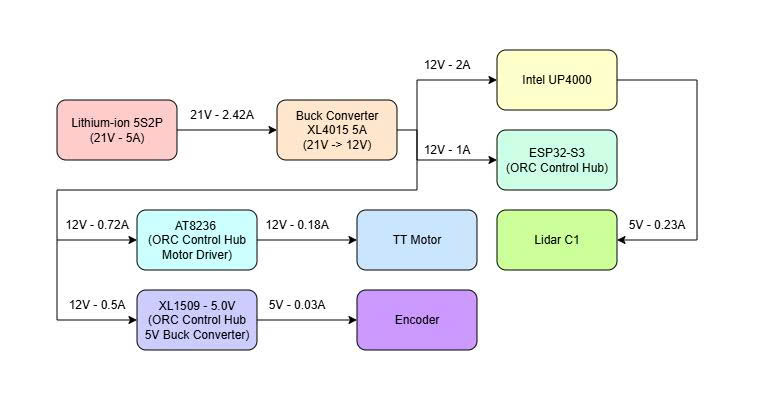
\includegraphics[width=0.9\textwidth]{Elec.jpg}
    \caption{Power distribution of the autonomous waiter robot.}
    \label{fig:power}
\end{figure}

\subsubsection{Mechanical Layout and Sensor Placement}
The robot is assembled on an Ohstem Beam X aluminum profile frame with approximate dimensions of $22.5\text{ cm} \times 16\text{ cm}$. Because the platform uses four Omni/Mecanum wheels, center-of-gravity placement directly affects wheel contact force and slippage. A balanced load distribution helps maintain predictable translational and rotational motion.

The LiDAR C1 is mounted on the highest tier of the robot so that its 360-degree scanning plane is not blocked by circuit boards or wiring. The UP 4000 is stacked below the LiDAR with mechanical standoffs that provide both clearance and passive cooling. The ORC Control hub controller is placed near the motors to shorten PWM and encoder wiring. The IMU is positioned as close as possible to the robot's center of rotation; otherwise, centripetal acceleration during spin motion can corrupt accelerometer measurements and reduce yaw-filter reliability. The battery is placed to counterbalance the front-heavy sensor and compute assembly.

\subsection{Low-Level Motion Control}
\subsubsection{Mecanum Kinematics}
The robot uses four omnidirectional Mecanum wheels. Compared with a differential drive, this configuration provides three planar degrees of freedom: longitudinal velocity $v_x$, lateral velocity $v_y$, and yaw velocity $\omega_z$. Inverse kinematics maps these body-frame commands to four motor commands.

In the ESP32 MicroPython - ORC Control hub firmware, ROS 2 velocity commands are scaled into integer motor commands. A simplified implementation is shown below.

\begin{lstlisting}[language=Python,caption={MicroPython - ORC Control hub implementation of inverse kinematics.},label={lst:kinematics}]
speed_x = int(vx * 180)
speed_y = int(vy * 180)
speed_w = int(wz * 180)

m1_speed = speed_x - speed_y - speed_w
m2_speed = speed_x + speed_y + speed_w
m3_speed = speed_x + speed_y - speed_w
m4_speed = speed_x - speed_y + speed_w

# Correct mirrored motor installation.
m1_speed = -m1_speed
m3_speed = -m3_speed

m1_speed = max(min(m1_speed, 100), -100)
m2_speed = max(min(m2_speed, 100), -100)
m3_speed = max(min(m3_speed, 100), -100)
m4_speed = max(min(m4_speed, 100), -100)
\end{lstlisting}

The sign correction for motors M1 and M3 compensates for mirrored physical installation. Saturation limits the command range to protect the motor driver and produce repeatable motion.

\subsubsection{Manual Teleoperation}
During mapping and calibration, manual control is required to move the robot through the environment while LiDAR and odometry data are collected. In this implementation, teleoperation is performed with a keyboard connected to the UP 4000. A ROS 2 teleoperation node running on the UP 4000 reads discrete key commands from the keyboard and converts them into body-frame velocity commands. The key layout follows a compact three-row pattern, where \texttt{u}, \texttt{i}, and \texttt{o} command diagonal-left forward, forward, and diagonal-right forward motion; \texttt{j}, \texttt{k}, and \texttt{l} command left motion, stop, and right motion; and \texttt{m}, \texttt{<}, and \texttt{>} command diagonal-left backward, backward, and diagonal-right backward motion. These commands are then sent from the UP 4000 to the ESP32-YOLO controller, which translates the requested $v_x$, $v_y$, and $\omega_z$ values into individual motor PWM signals through the Mecanum inverse-kinematic model. This keyboard-based workflow simplifies development because the operator can drive the robot, collect mapping data, and monitor ROS 2 topics from the same edge-computing platform.

\subsection{Odometry and Sensor Fusion}
\subsubsection{Mecanum Slippage}
Mecanum wheels provide excellent maneuverability but introduce significant slippage, especially during lateral motion and rapid rotation. If yaw is estimated only from encoder-based forward kinematics, angular drift accumulates quickly and can degrade SLAM. The implementation therefore uses a hybrid odometry strategy: encoder ticks estimate translational displacement, while the IMU provides the absolute yaw angle.

The encoder resolution is modeled as $11 \times 34 = 374$ pulses per wheel revolution. Raw telemetry contains encoder counts and yaw measurements, for example:

\begin{lstlisting}[language={},caption={Example MQTT telemetry payload.}]
{"e1": 1523, "e2": 1520, "yaw": 45.23}
\end{lstlisting}

\subsubsection{Euler Integration}
The bridge node receives telemetry at approximately 10 Hz. Wheel displacement is computed from tick differences:
\begin{align}
\Delta d_{left} &= \frac{\Delta ticks_{e1}}{N_{ppr}} \pi D_{wheel},\\
\Delta d_{right} &= \frac{\Delta ticks_{e2}}{N_{ppr}} \pi D_{wheel},\\
\Delta d_{center} &= \frac{\Delta d_{left} + \Delta d_{right}}{2}.
\end{align}

The global pose update uses the IMU heading $\theta_{IMU}$:
\begin{align}
X_t &= X_{t-1} + \Delta d_{center}\cos(\theta_{IMU}),\\
Y_t &= Y_{t-1} + \Delta d_{center}\sin(\theta_{IMU}).
\end{align}

This approach does not remove all Mecanum slip, but it reduces yaw drift and provides a more stable transform chain for SLAM Toolbox and Nav2.

\subsection{ROS 2 Foxy Deployment} 
\subsubsection{Operating System and Memory Optimization}
The UP 4000 is deployed in headless mode with Ubuntu Server 20.04 LTS. Avoiding a local graphical desktop reserves memory for ROS 2 nodes, SLAM, Nav2, and sensor processing. Since the device has only 2 GB of RAM, a 4 GB swap file is configured to prevent out-of-memory failures during package compilation.

\begin{lstlisting}[language=bash,caption={Swap configuration for the UP 4000.}]
sudo fallocate -l 4G /swapfile
sudo chmod 600 /swapfile
sudo mkswap /swapfile
sudo swapon /swapfile
\end{lstlisting}

\subsubsection{Workspace Organization}
The ROS 2 workspace is organized around description, bridge, simulation, and navigation packages. The description package contains URDF/Xacro files, meshes, and launch files. The bridge package translates microcontroller telemetry into ROS 2 topics. Simulation launch files spawn the robot in Gazebo and connect Gazebo topics to ROS 2. Navigation launch files start map loading, localization, costmaps, planners, controllers, and lifecycle management.

\subsection{Communication Bridge}

In a conventional ROS 2 architecture, a microcontroller can be integrated through micro-ROS so that it appears directly in the DDS network as an independent ROS node. However, this approach is too heavy for the ESP32-S3 ORC Control hub used in this project, especially when the controller is already running MicroPython. The limited heap memory available on the ESP32 makes a full micro-ROS client difficult to maintain reliably and may cause unstable execution during motor-control and sensor-acquisition tasks.

\subsubsection{Replacing micro-ROS}

The implemented architecture therefore replaces micro-ROS with a lightweight byte-stream bridge and an MQTT-based publish/subscribe channel. Instead of exchanging native ROS 2 messages on the microcontroller, the controller serializes commands and telemetry as raw JSON strings. These payloads can be transmitted through a serial link at 115200 baud or through an internal MQTT broker. In the deployed configuration, the MQTT broker \texttt{mqtt.ohstem.vn} on port \texttt{1883} is used as the intermediate communication layer between the ESP32 controller and the UP 4000 edge computer.

This design separates the low-level controller from the ROS 2 computation graph. If the edge computer is busy running SLAM, Nav2, or visualization-related processes, the microcontroller does not need to participate in DDS discovery or maintain a ROS 2 executor. As a result, motor-control timing and hardware-interrupt handling remain isolated from high-level operating-system delays.

\begin{figure}[htbp]
    \centering
    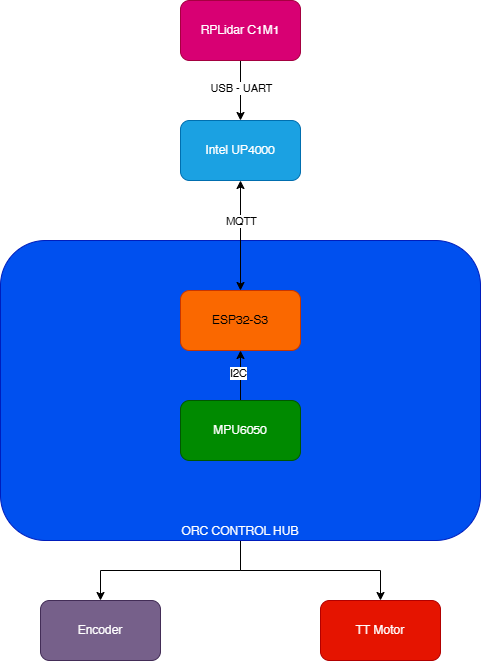
\includegraphics[width=0.5\textwidth]{Connect.png}
    \caption{Communication architecture.}
    \label{fig:Communication}
\end{figure}


\subsubsection{Bridge Node Logic}
A Python ROS 2 node named \texttt{waiter\_bridge\_node} acts as the translator between the ROS 2 topic ecosystem and the JSON-based physical communication layer. The node contains two main data paths: a downlink path from ROS 2 to the controller, and an uplink path from the controller back to ROS 2.

In the downlink path, the bridge subscribes to \texttt{/cmd\_vel} with a QoS history depth of 10. When Nav2 or the teleoperation node publishes a \texttt{geometry\_msgs/Twist} message, the callback function extracts the longitudinal velocity $v_x$, lateral velocity $v_y$, and yaw velocity $\omega_z$. These floating-point values are rounded to two decimal places and packed into a compact JSON command:

\begin{lstlisting}[language=Python,caption={JSON velocity command published by the bridge node.}]
{"vx": round(vx, 2), "vy": round(vy, 2), "wz": round(wz, 2)}
\end{lstlisting}

The resulting payload is published to the MQTT topic \texttt{210905/feeds/V3}. On the ESP32 side, the MicroPython firmware receives the UTF-8 JSON string, decodes it into velocity components, and passes the values to the Omni/Mecanum motor-control matrix.

In the uplink path, encoder counts and IMU yaw measurements are continuously sent from the physical robot to the MQTT broker. The bridge node runs the MQTT client loop in a separate daemon thread using \texttt{loop\_start()}, so MQTT communication does not block the ROS 2 executor. When a telemetry message arrives on \texttt{210905/feeds/V1}, the \texttt{on\_mqtt\_message} callback decodes the JSON payload, wraps the raw telemetry in a \texttt{std\_msgs/String} message, and publishes it to \texttt{/vehicle/telemetry}. The ROS 2 side can then consume this telemetry for odometry estimation, debugging, and transform publication.

\section{Simulation and Experimental Testing}
\subsection{URDF and Gazebo Simulation}
Before deployment on the physical chassis, the robot is represented as a digital twin in a simulation environment. This stage verifies the geometric model, the navigation logic, and the ROS 2 transform tree before the same software stack is connected to hardware.

\subsubsection{Robot Description}
The model is implemented in \texttt{robot.urdf.xacro}. It stores the geometric metadata of the robot and defines its links and joints in three-dimensional space. The core frame structure follows the physical dimensions of the Ohstem Beam X chassis. The \texttt{base\_footprint} frame represents the two-dimensional projection of the robot on the ground plane, while \texttt{base\_link} is placed at the physical center of the chassis with a vertical offset corresponding to the wheel radius.

\begin{figure}[htbp]
    \centering
    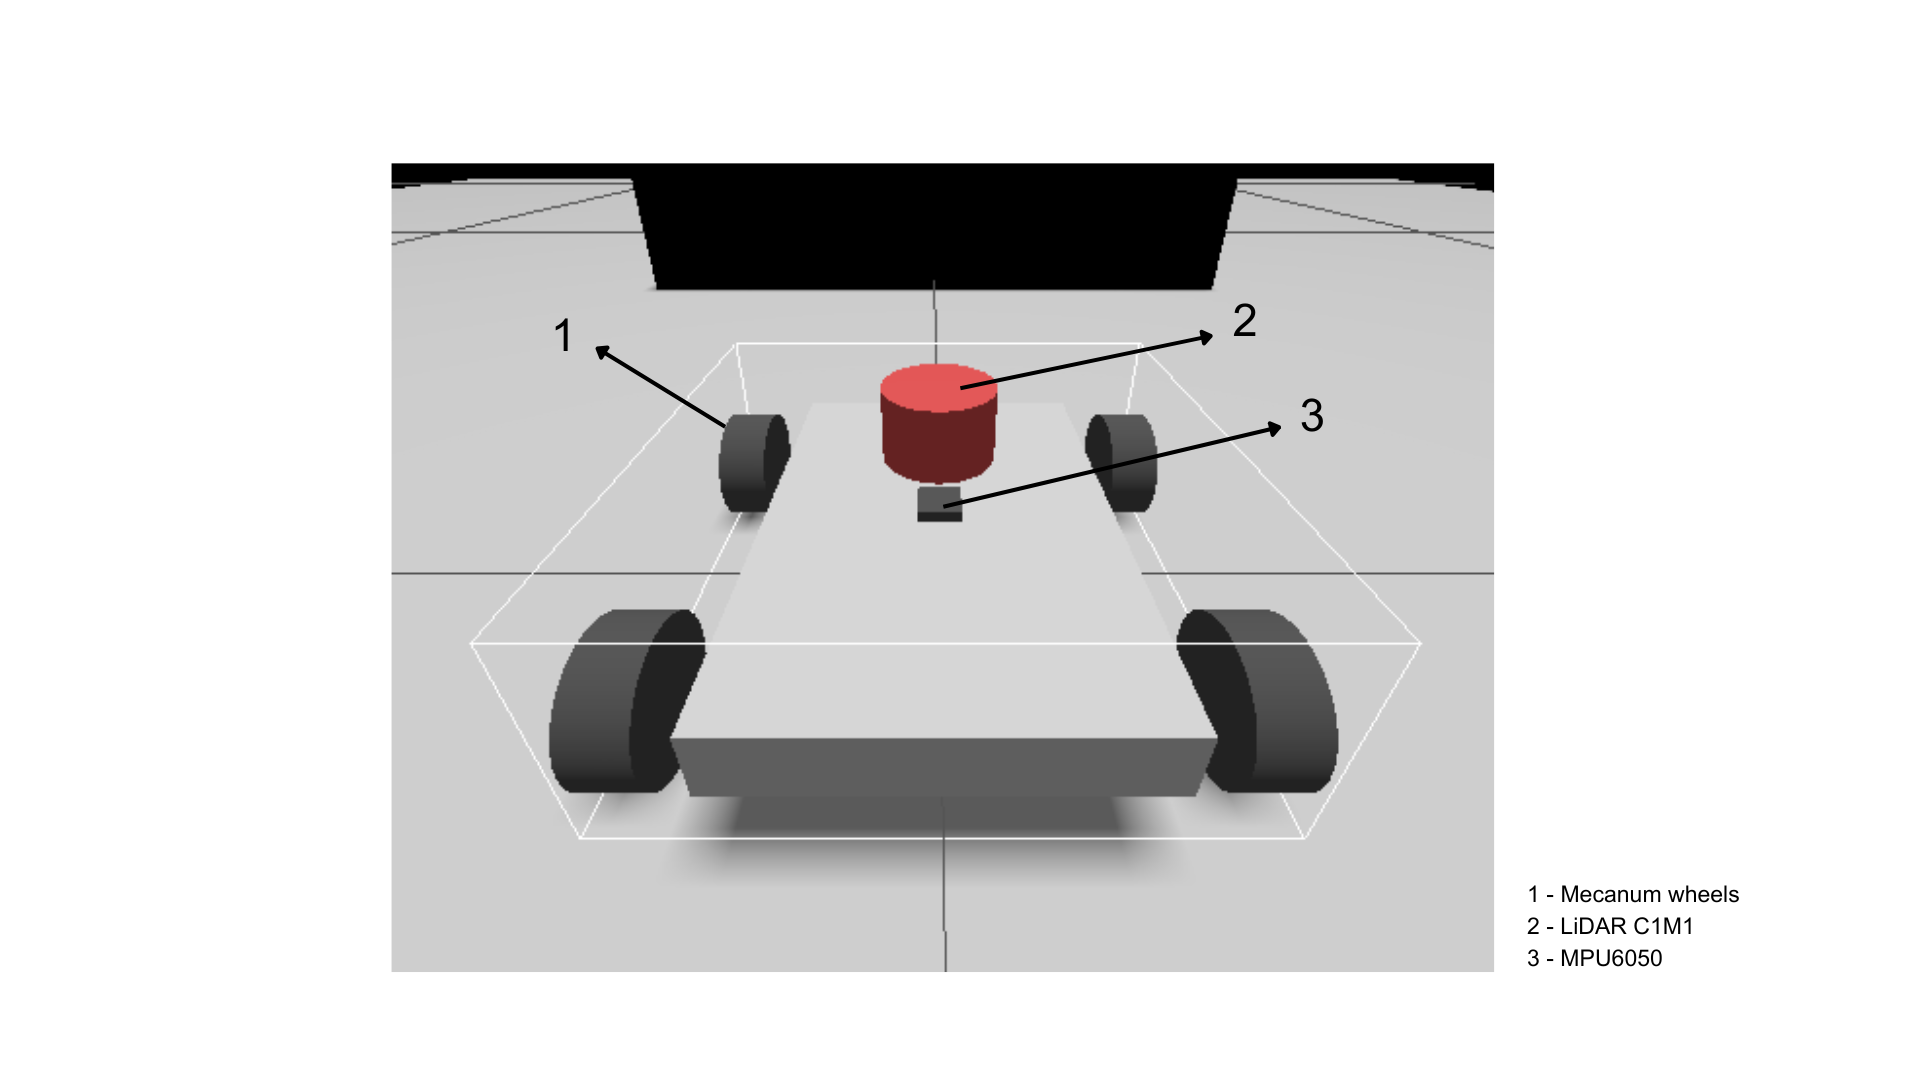
\includegraphics[width=1\textwidth]{Car.png}
    \caption{Robot Odometry in Gazebo.}
    \label{fig:gazebo_odometry}
\end{figure}

The Omni/Mecanum wheels are modeled differently from standard cylindrical wheels because their physical behavior includes intentional lateral slip. In the Gazebo model, wheel geometry, inertia parameters, and friction coefficients must be selected so that the simulated platform approximates the real sliding and strafing behavior of the Mecanum drive. Although the simulation cannot fully reproduce all contact effects of the roller structure, this model is sufficient for validating velocity commands, frame transforms, and navigation behavior.

The sensor transform tree is also defined in the robot description. The LiDAR C1 frame, named \texttt{laser\_frame}, is attached to the chassis through a fixed joint or an equivalent \texttt{static\_transform\_publisher}. It is placed above the robot with a positive $z$ translation that matches the mechanical mounting height, allowing ROS 2 nodes to interpret the scanning plane correctly. The IMU frame, named \texttt{imu\_link}, is attached near the center of \texttt{base\_link} so that accelerometer readings are less affected by centripetal acceleration during rotation. Correct frame placement is essential because SLAM and Nav2 depend on consistent transforms among \texttt{map}, \texttt{odom}, \texttt{base\_footprint}, \texttt{base\_link}, \texttt{laser\_frame}, and \texttt{imu\_link}.
\begin{figure}[htbp]
    \centering
    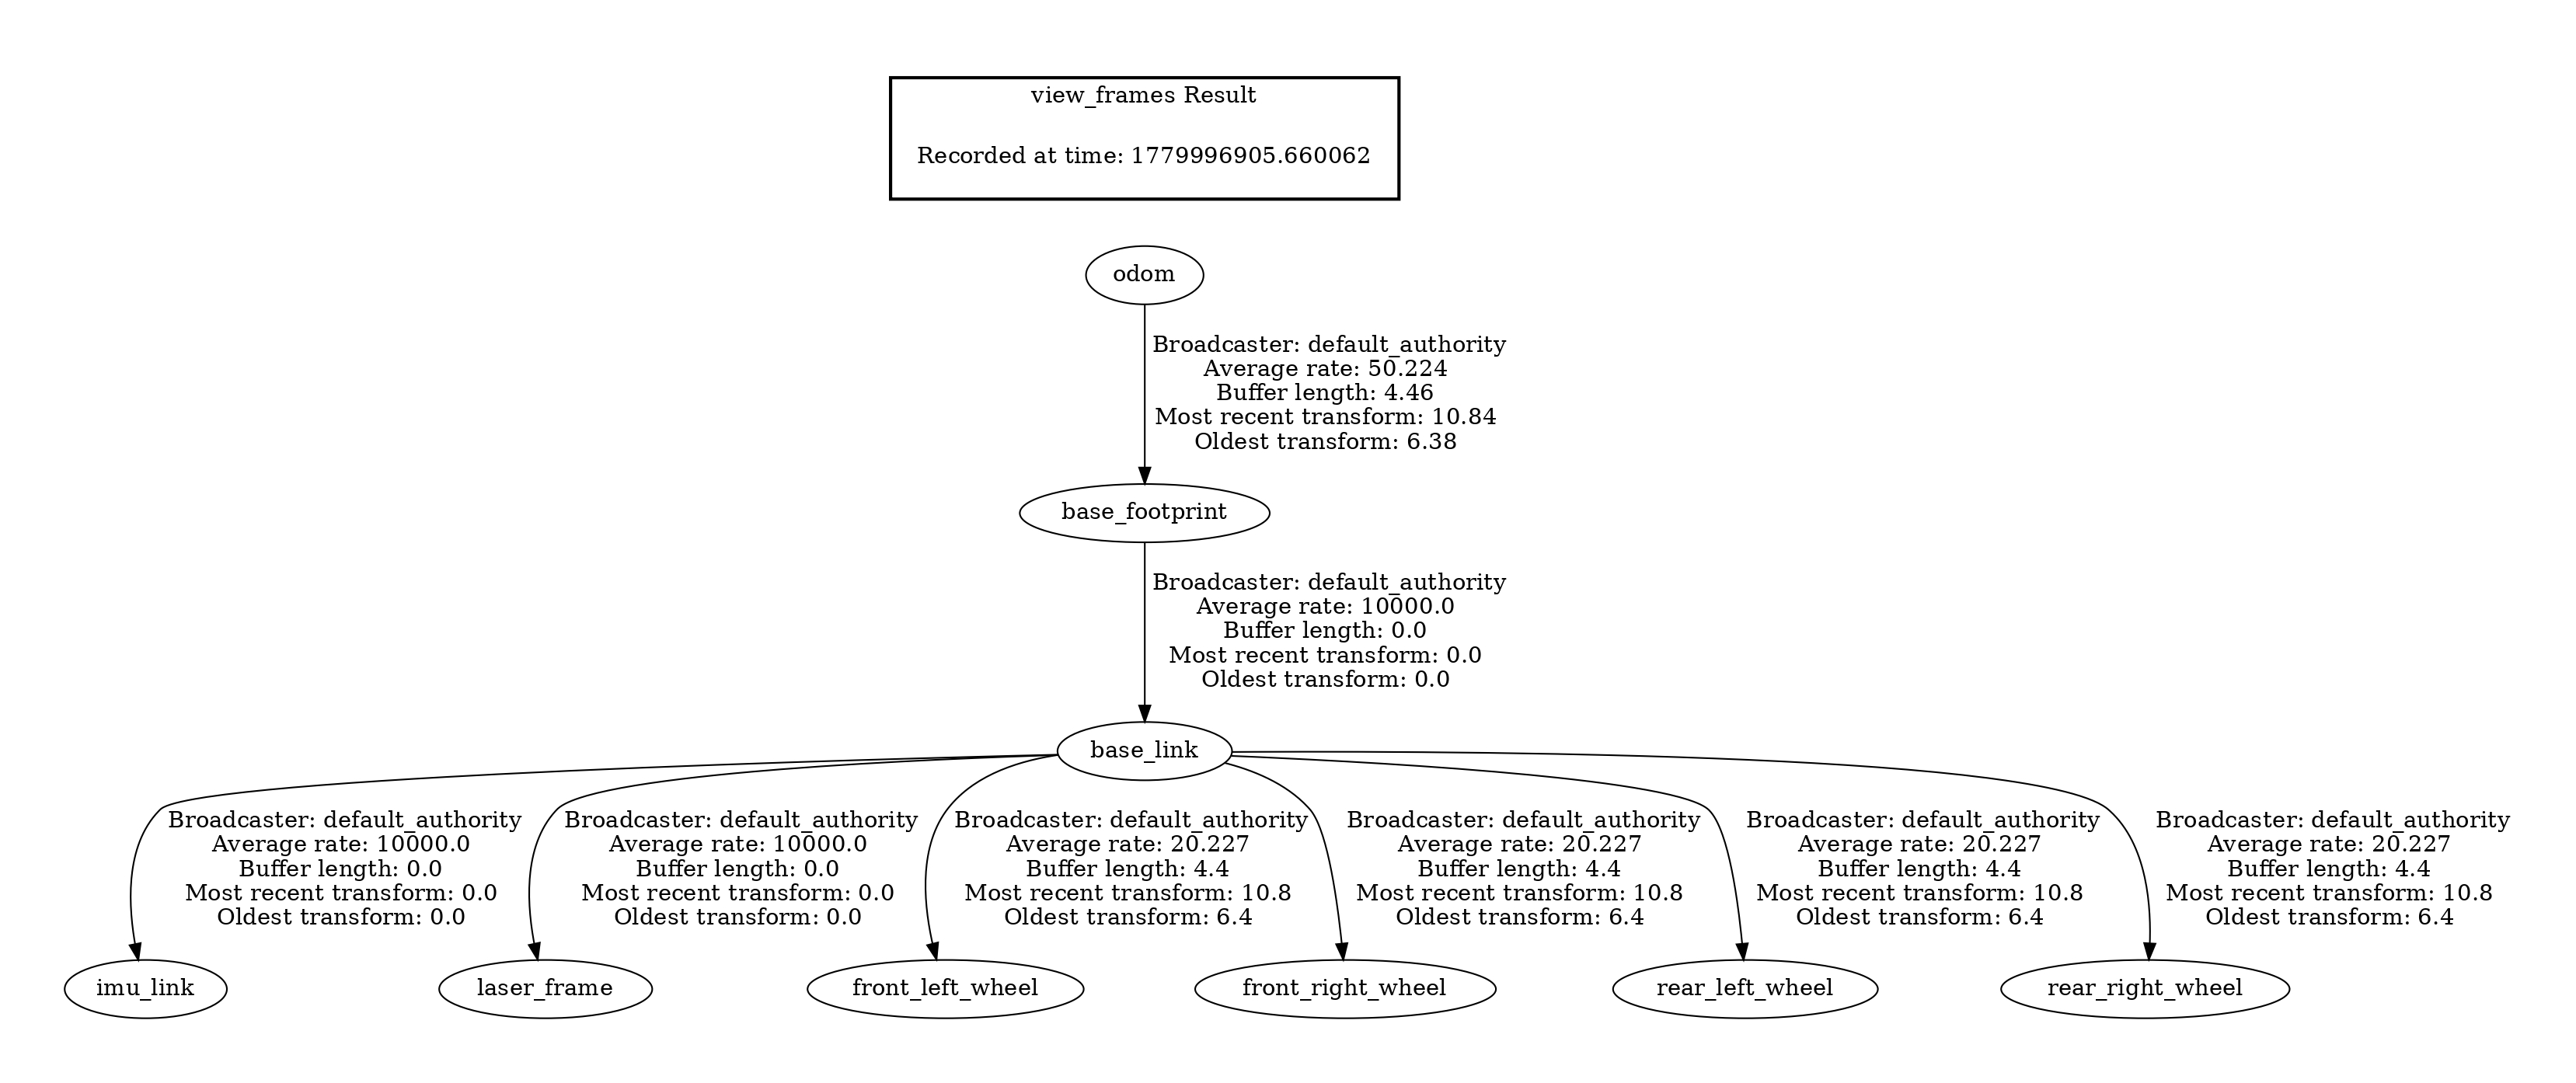
\includegraphics[width=\textwidth]{frame.jpg}
    \caption{ROS 2 TF transform tree of the robot sensor and base frames.}
    \label{fig:tf_transform_tree}
\end{figure}

\subsubsection{Gazebo and ROS-GZ Bridge}
The Gazebo launch process is organized around three main components. First, Robot State Publisher reads the URDF/Xacro model and publishes the robot kinematic structure to the ROS 2 TF network. This process provides the logical skeleton of the robot, including the base, wheels, LiDAR, and IMU frames. Second, the Gazebo server loads a static world file that represents the restaurant-like environment and spawns the robot entity at the selected initial pose. When simulation time is used, all ROS 2 nodes must be configured with \texttt{use\_sim\_time:=True}; otherwise, Nav2 and related algorithms may wait indefinitely for valid \texttt{/clock} messages. If the Gazebo world starts in a paused state, the operator must press Play in the simulator interface so that simulation time begins and the navigation stack becomes active.

Third, \texttt{ros\_gz\_bridge} connects the Gazebo transport layer with ROS 2 DDS communication. This bridge maps bidirectional topics such as \texttt{/scan}, \texttt{/tf}, \texttt{/clock}, and \texttt{/cmd\_vel} between the simulator and the ROS 2 graph. As a result, LiDAR data generated in Gazebo can be consumed by SLAM and Nav2, while velocity commands from ROS 2 can drive the simulated robot. During early testing, \texttt{teleop\_twist\_keyboard} can be launched from a terminal to send manual \texttt{/cmd\_vel} commands to the virtual robot, allowing the team to validate motion behavior and TF consistency before running the same control pipeline on the physical platform.

\subsection{SLAM and Navigation}
\subsubsection{SLAM Toolbox}

\begin{figure}[htbp]
    \centering
    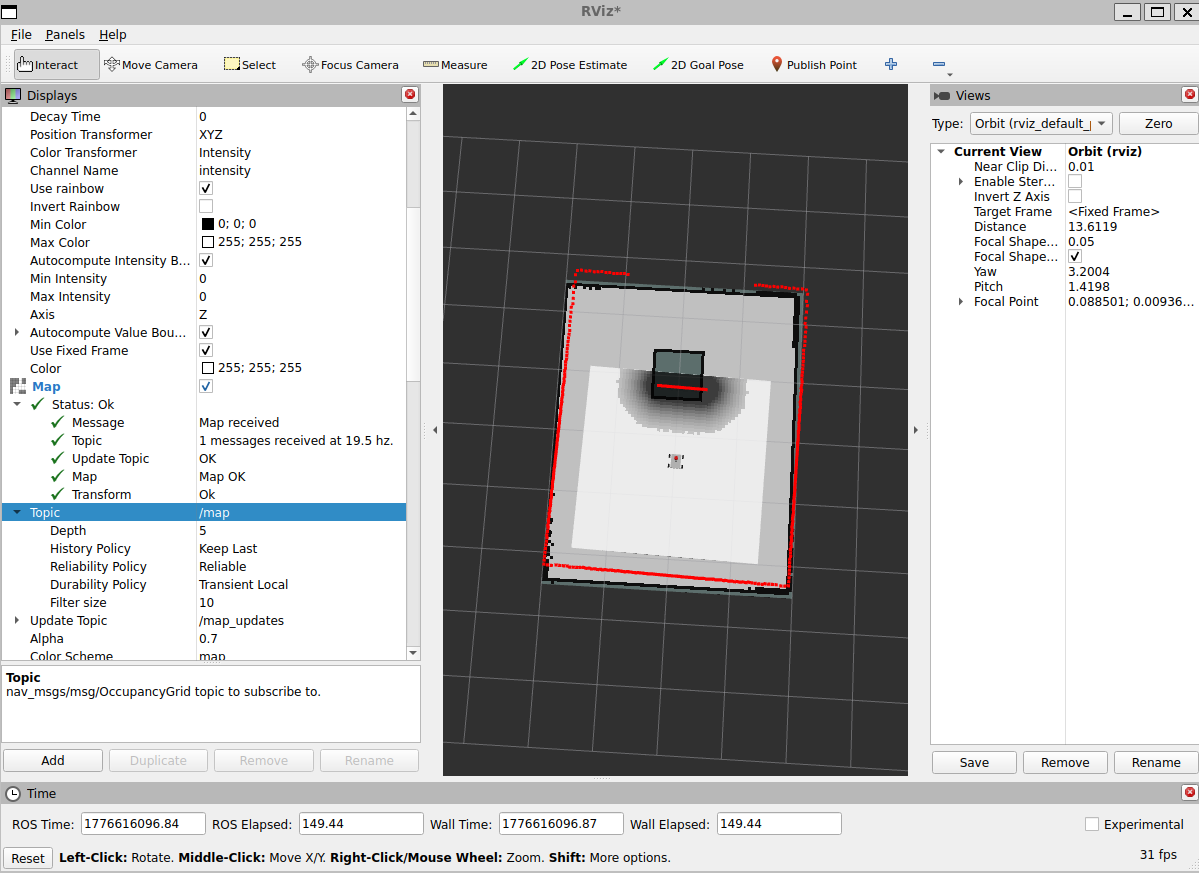
\includegraphics[width=0.8\textwidth]{Rviz2.png}
    \caption{Mapping in Rviz2.}
    \label{fig:Simulation Rviz2}
\end{figure}

The intelligent layer of the waiter robot is built around SLAM and Nav2. SLAM converts raw range measurements from the LiDAR into a spatial map, while Nav2 uses this map to produce feasible motion commands for autonomous navigation. In this project, mapping is performed using \texttt{slam\_toolbox}, a ROS 2 package based on 2D pose-graph SLAM.

The mapping process contains two main stages. In the front end, LiDAR C1 scan data published on \texttt{/scan} are aligned against previous scans and the partially built map. This scan-matching stage estimates the relative motion of the robot between successive observations. When the robot rotates or moves quickly, the IMU yaw measurement helps reduce scan distortion and improves the stability of the estimated pose.

In the back end, \texttt{slam\_toolbox} constructs a pose graph in which robot poses are represented as graph nodes and spatial constraints are represented as graph edges. Small odometry and scan-matching errors accumulate over time and may cause map drift, curved walls, or ghost obstacles. Pose-graph optimization reduces this accumulated error, especially when loop closure is detected. The Ceres Solver is used to solve the nonlinear optimization problem and adjust the pose graph so that repeated observations of the same corridor, wall, or intersection become geometrically consistent.

During practical testing, rapid manual rotation of the robot could still introduce light map artifacts. In these cases, clearing the local map buffer or restarting \texttt{slam\_toolbox} restored a clean mapping state quickly. After the room map was completed, it was saved as a static occupancy grid consisting of a \texttt{.yaml} metadata file and a \texttt{.pgm} map image.

\begin{figure}[htbp]
    \centering
    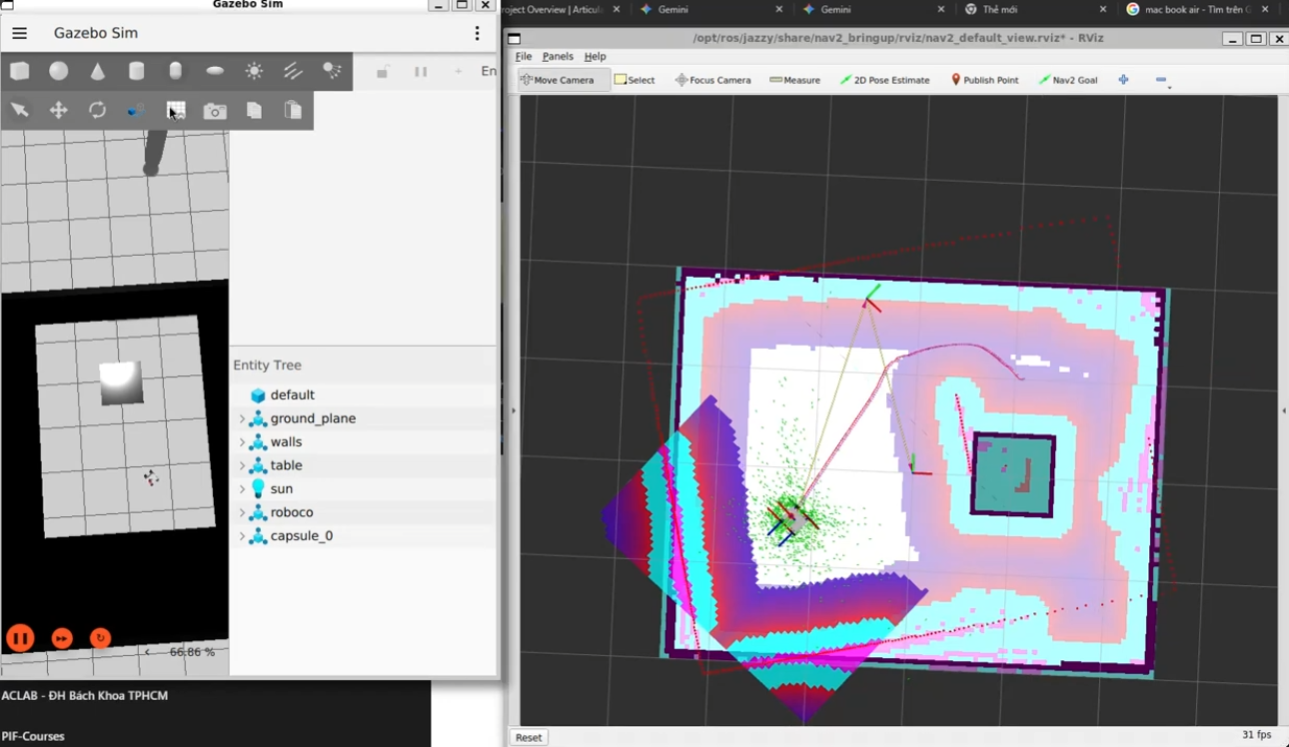
\includegraphics[width=0.8\textwidth]{simu.png}
    \caption{SLAM and Navigation in Gazebo and Rviz2.}
    \label{fig:Slam}
\end{figure}

\subsubsection{Nav2}
Navigation is implemented with the ROS 2 Navigation 2 stack. The launch file \texttt{navigation.launch.py} loads the saved map, such as \texttt{my\_room\_map.yaml}, using an absolute path to avoid missing-path errors during deployment. The Nav2 lifecycle nodes are configured with \texttt{autostart:=True}, allowing the navigation stack to activate automatically without requiring manual lifecycle transitions.

Localization is handled by AMCL, which estimates the robot pose on the static map using a particle filter. At startup, the robot does not yet know its exact position in the map frame, so the operator provides an initial pose in RViz2 using \texttt{2D Pose Estimate}. Once the LiDAR scan pattern converges with the stored wall and obstacle boundaries, AMCL produces a stable transform between \texttt{map}, \texttt{odom}, and \texttt{base\_link}. This transform is required before Nav2 can plan and execute navigation goals.

Nav2 uses two costmap layers for planning and obstacle avoidance. The global costmap represents the known static environment from the saved occupancy grid, while the local costmap updates around the robot using live LiDAR observations. Dynamic obstacles, such as people moving near the robot, are inserted into the local costmap. Inflation layers expand the occupied regions around obstacles, creating safety margins that discourage the planner and controller from selecting trajectories too close to walls, tables, or moving objects.

When the operator sends a \texttt{Nav2 Goal} in RViz2, a global planner such as NavFn or Smac computes a path across the global costmap. The local controller then converts this path into velocity commands on \texttt{/cmd\_vel}. Although the MPPI controller can produce smooth trajectories through sampling-based model predictive control, it requires more CPU and memory than the UP 4000 can comfortably provide. Therefore, the DWB Controller is used as the default local controller. DWB samples feasible velocity commands over a short time window and scores each trajectory according to goal progress, path alignment, and obstacle clearance. This provides a practical balance between navigation quality and computational cost on the 2 GB edge platform.


\section{Results and Discussion}
\subsection{Experimental Debugging and Optimization}
\subsubsection{USB Permission Failure}
During the transition from fixed power-supply testing to battery-powered operation at Checkpoint 4, the LiDAR C1 serial interface became one of the first system-level failure points. When the robot was powered from the independent 21 V lithium-ion battery pack, Ubuntu Server on the UP 4000 occasionally denied access to the USB serial device used by the LiDAR. As a result, ROS 2 LiDAR nodes produced timeout errors such as \texttt{RESULT\_OPERATION\_TIMEOUT 80008004}, and the \texttt{laser\_frame} data stream was interrupted. This failure directly affected the TF chain and prevented SLAM and Nav2 from receiving valid scan data.

The immediate workaround was to manually grant read and write access to the USB serial device:

\begin{lstlisting}[language=bash]
sudo chmod 666 /dev/ttyUSB0
\end{lstlisting}

This command restored LiDAR communication and allowed scan data to flow into the ROS 2 graph again. However, this solution is temporary because the device name and permission state may change after reconnection or reboot. For a stable deployment, a dedicated udev rule should be configured so that the LiDAR always receives a persistent device name and the correct access permissions.

\subsubsection{MQTT Topic and Odometry Errors}
A second major issue appeared in the odometry pipeline. The Yolo Uno/ORC controller continued publishing encoder and IMU telemetry to the MQTT broker, but the \texttt{waiter\_bridge\_node} on the UP 4000 did not receive the expected messages. The root cause was a mismatch between the topic path published by the MQTT client library and the topic path subscribed to by the bridge node. In practice, the client library inserted an additional topic prefix, so the telemetry stream was present on the broker but invisible to the ROS 2 bridge.

This mismatch caused the robot pose to remain fixed at the origin even while the physical robot was moving. Additional Python issues made the symptom worse: early patches contained indentation errors in the Euler integration block and hard-coded zero velocity values, so the odometry update could not propagate displacement into the ROS 2 TF tree. Consequently, SLAM Toolbox and Nav2 reported transform-related failures such as missing transforms from \texttt{base\_link} to \texttt{map}.

The debugging process used MQTT Explorer to inspect the live broker hierarchy and identify the actual telemetry topic. After the bridge subscription was redirected to the correct path, such as \texttt{210905/feeds/V1}, encoder counts and IMU yaw values reached the UP 4000 again. The Python bridge was then corrected so that the Euler integration used the received yaw angle and encoder displacement instead of fixed zero values. This restored the odometry stream and allowed the ROS 2 transform chain to update continuously.

\subsubsection{Distributed Visualization}
The third challenge came from the limited 2 GB RAM capacity of the UP 4000. Running Gazebo or RViz2 directly on the edge computer consumed too much memory and reduced the reliability of navigation nodes. The final workflow therefore adopted a distributed visualization architecture. Heavy computation related to AMCL, SLAM Toolbox, Nav2, costmaps, and TF publication runs headlessly on the robot, while graphical monitoring is moved to a Windows workstation connected to the same local Wi-Fi network and ROS 2 DDS domain.

In this configuration, the Windows workstation launches the RViz2 navigation view and subscribes to the robot's ROS 2 topics over the network. This allows the operator to inspect LiDAR scans, TF axes, the occupancy grid map, and costmap layers in real time without loading the UP 4000 with 3D rendering tasks. The same workstation is also used to provide the initial pose through \texttt{2D Pose Estimate} and to send autonomous navigation goals through \texttt{Nav2 Goal}.

During integration, a duplicated \texttt{robot\_state\_publisher} entry in the RViz/navigation launch configuration caused visual flickering and redundant TF publication. Removing this duplicate publisher reduced unnecessary network traffic and stabilized the displayed robot model. Overall, distributed visualization preserved edge-computer memory while maintaining a practical debugging and operation interface for the robot.

A demonstration video is available online: \href{https://youtu.be/hw2yS5E_YpA?si=joVXpEF2XMeXMV-6}{Waiter Robot demonstration video}.

\section{Conclusions}
This paper has presented a systematic design and implementation study of a modern autonomous waiter robot based on ROS 2 Jazzy(Windown PC) and ROS 2 Foxy(UP4000). The work shows that a low-cost hardware platform can still support practical indoor service-robot functions when the mechanical structure, power system, embedded controller, edge computer, and ROS 2 software stack are designed as a unified architecture. Key hardware limitations, including Mecanum-wheel odometry uncertainty and the restricted 2 GB memory capacity of the UP 4000 edge computer, were addressed through coordinated hardware and software decisions.

The proposed platform combines separated power distribution, balanced Beam X mechanical placement, Mecanum inverse kinematics, encoder-IMU odometry, and Euler pose integration to improve motion stability and localization consistency. On the communication side, the lightweight JSON/MQTT bridge replaces a heavier micro-ROS architecture and reduces the computational burden on the ESP32-S3 controller. On the edge computer, Ubuntu Server deployment, swap configuration, and distributed visualization make it possible to run ROS 2 Jazzy, SLAM Toolbox, Gazebo-based validation, and Nav2 navigation with the DWB Controller under constrained memory conditions.

Future work will extend the robot with camera-based perception, including USB camera streaming and a lightweight YOLOv5n model for object recognition. ArUco marker detection can also be integrated to support table identification, docking, and task interaction in restaurant environments. In addition, a customer-facing graphical user interface and an audio feedback module will improve human-robot interaction and operational safety. These extensions can build on the current modular architecture and further demonstrate the potential of low-cost embedded platforms for autonomous service robots.

\begin{thebibliography}{10}

\bibitem{pmc_ros2_kubernetes_2025}
Li, X., et al.: Enhancing the Resilience of ROS 2-Based Multi-Robot Systems with Kubernetes: A Case Study on UWB-Based Relative Positioning. \emph{Sensors (Basel)}, 25(2) (2025). \url{https://pmc.ncbi.nlm.nih.gov/articles/PMC12390455/}

\bibitem{ieee_microros_attitude_2023}
Author, et al.: Implementation and Performance Study of the Micro-ROS/ROS2 Framework to Algorithm Design for Attitude Determination and Control System. \emph{IEEE Transactions} (2023). \url{https://www.researchgate.net/publication/375437006_Implementation_and_Performance_Study_of_the_Micro-ROSROS2_Framework_to_algorithm_design_for_Attitude_Determination_and_Control_System}

\bibitem{cambridge_mecanum_2016}
Lynch, K. M., Park, F. C.: Wheeled Mobile Robots. In: \emph{Modern Robotics: Mechanics, Planning, and Control}, pp. 445--489. Cambridge University Press (2017). \url{https://modernrobotics.northwestern.edu/nu-gm-book-resource/13-2-omnidirectional-wheeled-mobile-robots-part-1-of-2/}

\bibitem{mdpi_robust_slam_2021}
Wu, J., et al.: Robust Tightly Coupled Pose Measurement Based on Multi-Sensor Fusion in Mobile Robot System. \emph{Sensors}, 21(16), 5522. MDPI (2021). \url{https://www.mdpi.com/1424-8220/21/16/5522}

\bibitem{up4000} 
UP Board: UP 4000 Edge | AI-Powered Edge Computing for IoT Solutions. \url{https://up-board.org/up-4000/}

\bibitem{nav2_dwb} 
ROS 2 Documentation: DWB Controller — Nav2 1.0.0 documentation. \url{https://docs.nav2.org/configuration/packages/configuring-dwb-controller.html}

\end{thebibliography}

\end{document}
